\documentclass[t,aspectratio=169]{beamer} % 使用16:9宽高比
\usetheme{Madrid} % 选择Madrid主题
\usecolortheme{default} % 使用默认颜色主题

% 设置字体
\usepackage[UTF8]{ctex}
\usefonttheme{structurebold} % 加粗结构字体

% 数学包
\usepackage{amsmath, amssymb, bm}
\usepackage{url}
\usepackage{booktabs}

% 图形包
\usepackage{graphicx}

% 标题页信息
\title[9.3.学习曲线]{第9章：正则化}
\subtitle{第3节：学习曲线 (Learning Curves)}
\author{《深度学习基础》课程小组}
% \institute{上海立信会计金融学院}
\date{\today}

\begin{document}

% 标题页
\frame{\titlepage}

% 目录页
\begin{frame}
    \frametitle{目录}
    \tableofcontents
\end{frame}

% ============================================================
% 第一部分：学习曲线基础
% ============================================================
\section{学习曲线基础}

\begin{frame}
    \frametitle{1. 学习曲线：训练过程的可视化}
    \begin{itemize}
        \item 泛化性能受多种因素影响：
        \begin{itemize}
            \item 模型参数数量
            \item 数据集大小
            \item 权重衰减正则化系数
        \end{itemize}
        \item 每个因素都在\alert{偏差-方差}之间进行权衡。
        \item 另一个影响权衡的因素：\alert{学习过程本身}。
        \item 梯度下降优化中：
        \begin{itemize}
            \item 训练误差通常随参数更新而\alert{下降}
            \item 留出数据误差可能\alert{非单调}
        \end{itemize}
        \item \alert{学习曲线}：绘制训练集和验证集误差随迭代次数的变化。
        \item 提供训练进展的洞察，以及控制有效模型复杂度的实用方法。
    \end{itemize}
\end{frame}

% ============================================================
% 第二部分：早停法
% ============================================================
\section{早停法}

\begin{frame}
    \frametitle{2. 早停法 (Early Stopping)}
    \begin{itemize}
        \item 控制网络有效复杂度的另一种方法。
        \item 深度学习训练：迭代减少训练集上的误差函数。
        \item \textbf{典型行为}：
        \begin{itemize}
            \item 训练集误差：随迭代次数\alert{大致单调下降}
            \item 验证集误差：\alert{先下降，后上升}（网络开始过拟合）
        \end{itemize}
        \item \textbf{策略}：在验证集误差\alert{最小点}停止训练。
    \end{itemize}
    \begin{figure}
        \centering
        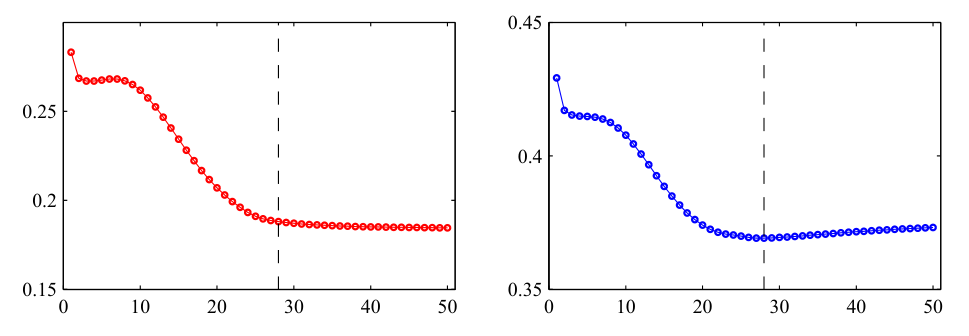
\includegraphics[width=0.5\textwidth]{figure-9-7.png}
        \caption{训练集误差（左）和验证集误差（右）随迭代步数的变化。}
    \end{figure}
\end{frame}

\begin{frame}
    \frametitle{2.1 早停法与有效参数数量}
    \begin{itemize}
        \item 学习曲线行为可用\alert{有效参数数量}定性解释。
        \item 有效参数数量：
        \begin{itemize}
            \item 训练开始时\alert{较小}
            \item 随训练\alert{增长}
            \item 对应模型有效复杂度的稳定增加
        \end{itemize}
        \item 在训练误差达到最小值之前停止训练 = 限制有效模型复杂度。
    \end{itemize}
\end{frame}

\begin{frame}[allowframebreaks]
    \frametitle{2.2 早停法与权重衰减的等价性}
    对二次误差函数，早停法与简单权重衰减\alert{行为相似}（Bishop, 1995a）。
    \begin{figure}
        \centering
        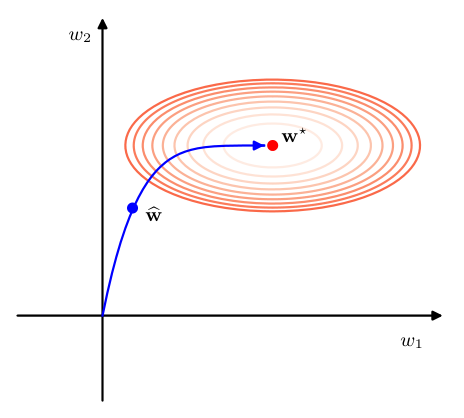
\includegraphics[width=0.3\textwidth]{figure-9-8.png}
        \caption{早停法为何能给出与权重衰减相似的结果。}
    \end{figure}
    \begin{itemize}
        \item 权重空间坐标轴旋转以对齐海森矩阵特征向量。
        \item 无权重衰减时，权重从原点出发沿负梯度方向移动：
        \begin{itemize}
            \item 先平行于 $w_2$ 轴移动，经过 $\bar{\mathbf{w}}$ 附近
            \item 然后移向误差函数最小值 $\mathbf{w}_{\text{ML}}$
        \end{itemize}
        \item 在 $\bar{\mathbf{w}}$ 附近停止 $\approx$ 权重衰减。
        \item \alert{关键关系}：$\tau/\eta$ 类似于正则化参数 $\lambda$ 的倒数。
        \item 有效参数数量在训练过程中\alert{增长}。
    \end{itemize}
\end{frame}

% ============================================================
% 第三部分：双下降
% ============================================================
\section{双下降}

\begin{frame}
    \frametitle{3. 双下降 (Double Descent)}
    \begin{itemize}
        \item 经典偏差-方差权衡：
        \begin{itemize}
            \item 参数太少：高偏差，测试误差大
            \item 参数增加：测试误差\alert{下降}
            \item 参数过多：高方差，测试误差\alert{再次上升}
        \end{itemize}
        \item 经典统计学的传统观念：模型参数数量需根据数据集大小限制。
        \item \textbf{但现代深度神经网络相反}：
        \begin{itemize}
            \item 即使参数数量\alert{远超}完美拟合训练数据所需，仍能表现优异。
            \item 深度学习界的普遍智慧：\alert{更大的模型更好}。
            \item 模型可训练到零误差，仍能在测试数据上表现良好。
        \end{itemize}
    \end{itemize}
\end{frame}

\begin{frame}
    \frametitle{3.1 双下降现象}
    \begin{itemize}
        \item 看似矛盾的现象可通过\alert{双下降}调和（Belkin et al., 2019）。
        \item 图 9.9：ResNet18 在图像分类任务上的训练集和测试集误差 vs 模型复杂度。
        \item \textbf{观察}：
        \begin{itemize}
            \item 训练误差：随复杂度增加\alert{单调下降}
            \item 测试误差：先下降，再上升，\alert{最后再次下降}
            \item 即使训练误差达到零后，测试误差仍继续下降
        \end{itemize}
    \end{itemize}
    \begin{figure}
        \centering
        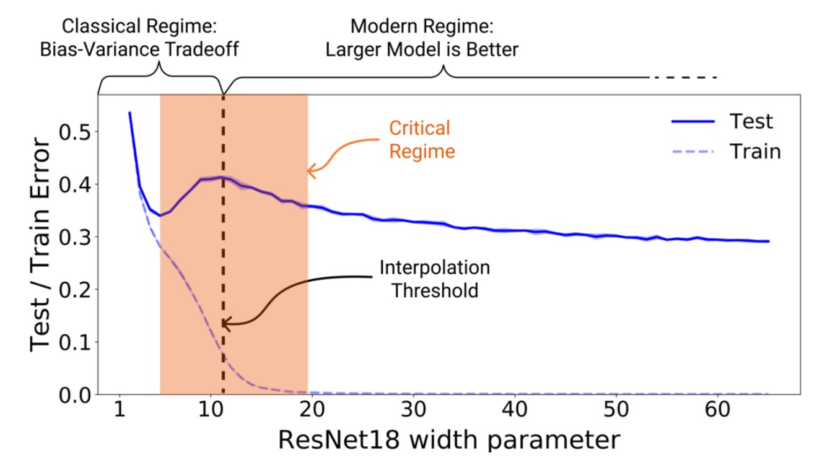
\includegraphics[width=0.3\textwidth]{figure-9-9.png}
        \caption{ResNet18 的训练误差与测试误差 vs 模型复杂度。}
    \end{figure}
\end{frame}

\begin{frame}
    \frametitle{3.2 双下降的两个区域}
    \begin{itemize}
        \item 比经典偏差-方差讨论更复杂，展现\alert{两个不同区域}：
        \begin{enumerate}
            \item \alert{经典区域}（小到中等复杂度）：经典偏差-方差权衡。
            \item \alert{现代区域}（非常大模型）：测试误差进一步下降。
        \end{enumerate}
        \item 两区域过渡大致发生在：
        \begin{itemize}
            \item 模型参数足够多，能够\alert{精确拟合训练数据}。
        \end{itemize}
        \item Nakkiran et al. (2019) 定义\alert{有效模型复杂度}：
        \begin{itemize}
            \item 模型能实现零训练误差的\alert{最大训练集大小}。
            \item 双下降出现在有效模型复杂度\alert{超过训练集数据点数}时。
        \end{itemize}
    \end{itemize}
\end{frame}

\begin{frame}
    \frametitle{3.3 早停法与双下降}
    \begin{itemize}
        \item 用\alert{早停法}控制模型复杂度时也观察到类似行为（图 9.10）。
        \item 增加训练轮数 $\Rightarrow$ 增加有效模型复杂度。
        \item 对足够大的模型，再次观察到双下降。
        \item 此类模型有许多可能解，包括\alert{过拟合}的解。
        \item 似乎是\alert{随机梯度下降}的隐式偏置导致良好泛化性能。
    \end{itemize}
    \begin{figure}
        \centering
        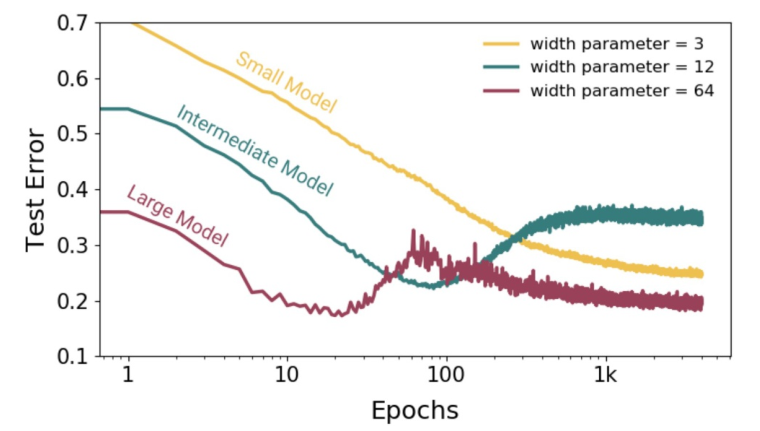
\includegraphics[width=0.3\textwidth]{figure-9-10.png}
        \caption{ResNet18 的测试误差 vs 训练轮数。}
    \end{figure}
\end{frame}

\begin{frame}
    \frametitle{3.4 正则化与双下降}
    \begin{itemize}
        \item 用\alert{正则化项}控制复杂度时也有类似结果。
        \item 大模型训练至收敛的测试误差 vs $1/\lambda$（正则化参数倒数）：
        \begin{itemize}
            \item 高 $\lambda$ $\Rightarrow$ 低复杂度
            \item 观察到\alert{双下降}现象（Yilmaz and Heckel, 2022）
        \end{itemize}
    \end{itemize}
    \begin{block}{核心洞察}
        双下降是\alert{模型复杂度与泛化性能}关系的更完整描述。\\
        经典偏差-方差权衡只是其中一部分。
    \end{block}
\end{frame}

\begin{frame}
    \frametitle{3.5 双下降的反直觉推论}
    \begin{itemize}
        \item \alert{讽刺性推论}：可能存在增加训练数据反而\alert{降低性能}的区域。
        \item 与传统观点“更多数据总是好事”相反。
        \item 对处于\alert{临界区域}的模型：
        \begin{itemize}
            \item 增加训练集大小可能将插值阈值\alert{向右推}。
            \item 导致更高的测试集误差。
        \end{itemize}
        \item 图 9.11：Transformer 模型测试误差 vs 嵌入维度。
        \begin{itemize}
            \item 训练集从 4,000 增加到 18,000：整体曲线大幅下降。
            \item 但对某些中间嵌入维度（临界复杂度区域），增加数据量反而\alert{降低泛化性能}。
        \end{itemize}
    \end{itemize}
    \begin{figure}
        \centering
        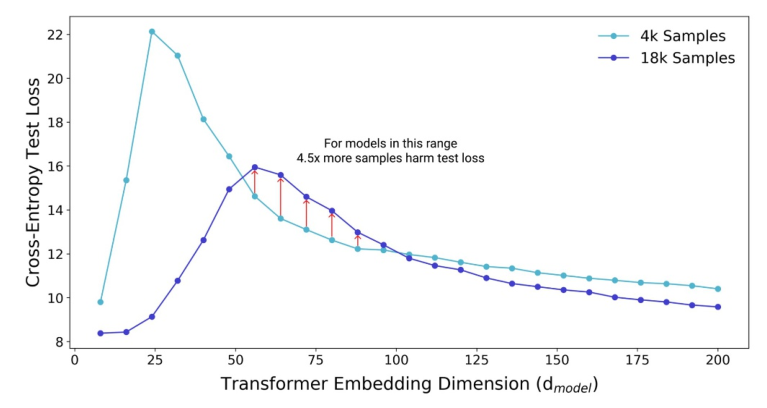
\includegraphics[width=0.25\textwidth]{figure-9-11.png}
        \caption{Transformer 模型的测试误差 vs 嵌入维度。}
    \end{figure}
\end{frame}

% ============================================================
% 第四部分：总结
% ============================================================
\section{总结}

\begin{frame}
    \frametitle{4. 本节总结}
    \begin{itemize}
        \item \alert{学习曲线}：训练集和验证集误差随迭代次数的变化。
        \item \alert{早停法}：
        \begin{itemize}
            \item 在验证集误差最小点停止训练。
            \item 有效参数数量在训练中增长。
            \item 与权重衰减相似：$\tau/\eta \sim 1/\lambda$。
        \end{itemize}
        \item \alert{双下降}：
        \begin{itemize}
            \item 测试误差 vs 模型复杂度：先降、再升、\alert{最后再降}。
            \item 两个区域：经典偏差-方差区域 + 现代大模型区域。
            \item 过渡点：模型刚好能\alert{精确拟合训练数据}。
            \item 有效模型复杂度超过训练集大小时出现。
        \end{itemize}
        \item \alert{反直觉推论}：临界区域增加数据可能降低性能。
        \item \alert{SGD 的隐式偏置}：即使模型可过拟合，SGD 仍导致良好泛化。
        \item 现代深度学习：\alert{更大模型往往更好}，与经典统计学观念不同。
    \end{itemize}
\end{frame}

% ============================================================
% 第五部分：参考文献
% ============================================================
\section{参考文献}

\begin{frame}
    \frametitle{5. 参考文献}
    \begin{itemize}
        \item 教材：Bishop, C. M. \& Bishop, H. (2023). Deep Learning Foundations and Concepts. Springer Nature Switzerland AG.
        \item Bishop, C. M. (1995a). Regularization and complexity control in feed-forward networks.
        \item Belkin, M. et al. (2019). Reconciling modern machine-learning practice and the classical bias--variance trade-off.
        \item Nakkiran, P. et al. (2019). Deep double descent: Where bigger models and more data hurt.
        \item Zhang, C. et al. (2016). Understanding deep learning requires rethinking generalization.
        \item Yilmaz, F. F. \& Heckel, R. (2022). Regularization-wise double descent.
    \end{itemize}
\end{frame}

\end{document}